\documentclass[12pt,twoside]{article}
% \documentclass{article}
% \date{}   %uncommenting this erases the date

\usepackage[utf8]{inputenc}
\usepackage{subfiles}

\usepackage{graphicx}
\usepackage{amsmath}
\usepackage{amssymb}
\usepackage{natbib}
\usepackage{verbatim}
\usepackage{floatpag}
\usepackage{subeqnarray}
\usepackage{mathrsfs}    %for special characters
\usepackage{cancel}  % to set terms in an equation to zero

\usepackage{hyperref}

\usepackage{amsthm}

\setlength{\textheight}     {9.0in}
\setlength{\textwidth}      {6.5in}
\setlength{\oddsidemargin}  {0.0in}
\setlength{\evensidemargin} {0.0in}
\setlength{\topmargin}      {0.0in}
\setlength{\headheight}     {0.0in}
\setlength{\headsep}        {0.0in}
\setlength{\hoffset}        {0.0in}
\setlength{\voffset}        {0.0in}
\setlength{\parindent}      {0.0in}      %starting new line at extreme left

\graphicspath{{Figures/}}



\newtheorem{lemma}{Lemma}
\newtheorem{thm}{Theorem}
\newtheorem{prop}{Proposition}

\usepackage{bbm}
\usepackage{algorithmic}

\begin{document}
\title{Gradient Flow Optimizers}
\author{Raghav K. Singhal}
\maketitle

%!TEX root=./optim_report.tex
\section{Introduction}
In this paper we present a new optimization method, which is based on the idea that Gradient Descent is a Euler Approximation to the solution of the following Ordinary Differential Equation:
\begin{equation}\label{gradFlow}
\dot{x}_t = -\nabla_{x}f(x_t)
\end{equation}
The Euler Approximation to this Ordinary Differential Equation is of the following form:
\begin{align*}
x_{n+1} =  x_n - \alpha \nabla_{x}f(x_n)
\end{align*}
where $\alpha$ is the step-size and in the Optimization Literature is referred to as the Learning Rate. In recent years there has been some interest in analyzing Optimzation Schemes using Differential Equation \cite{su2014}, etc.
\\
\\
Note \cite{su2014} uses a second-order differential equation to analyze Nesterov's Accelerated Gradient Descent, but it reverse-engineers a Differential Equation to analyze a particular method. We take the forward approach of first motivating the Ordinary Differential Equation point of view and then deriving optimization schemes, an approach already taken by \cite{alex2017}, where they analyze linear-multistep methods and other methods for integration of Differential Equations and analyze their performance as Optimization Schemes. We look at a very famous and stable class of optimizers, Runge-Kutta Methods, and compare their performance with Gradient Descent, AdaGrad, Stochastic Gradient Descent, SGD with momentum and Accelerated Stochastic Gradient Descent.
\\
\\
However, the goal in each field is different, in Optimization we look at an infinite-time horizon to find an approximation close to a global or a local minima but in Numerical Analysis of Differential Equations, the goal is to find a close approximation to the solution of the Differential Equation over a finite time interval $[0, T]$. But we try to bridge this gap by saying that the the solution trajectory for \eqref{gradFlow} stays close if not converges to the critical points of $f$, and we formalize this view by noting that the critical points of the loss function $f(x)$ are also the $\omega$-limit points of the \eqref{gradFlow}.
\\
\\
\section{Motivation}
Here we provdide certain properties of the solution of \eqref{gradFlow}, when $f \in \mathcal{S}^{2,1}_{\mu,\beta}(\mathbb{R}^n)$, that is $f$ is strongly convex and twice differentiable with $|| \nabla f(x) - \nabla f(y) || \leq \beta ||x - y||$, for all $x,y \in \mathbb{R}^n$ and $f$ is $\mu$-strongly convex. Then note that $\forall t >0$:
\begin{equation}
\begin{aligned}
\frac{d}{dt}\big(f(x_t) - f(x^*) \big) &= \left\langle \nabla f(x_t), \dot{x}_t \right\rangle \\
& = - ||\nabla f(x_t)||_2^2
\end{aligned}
\end{equation}
% Now, note that $|| \nabla f(x) || \leq \beta || x - x^* ||$, which implies that
% \begin{equation}
% \begin{aligned}
% - \beta^2 || x_t - x^* || \leq -||\nabla f(x_t)||_2^2 = \frac{d}{dt}\big(f(x_t) -f(x^*)\big) \\
% \frac{d}{dt} \big(f(x_t) - f(x^*) \big) \geq \beta || x_t - x^* ||_2^2
% \end{aligned}
% \end{equation}
But, as $f(x_t)\in \mathcal{S}^{2,1}_{\mu,\beta}(\mathbb{R}^n)$, we have that:
\begin{equation}
\begin{aligned}
f(x) - f(x^*) \leq \frac{1}{2\mu}|| \nabla f(x)||_2^2
\end{aligned}
\end{equation}
Hence,
\begin{equation}
\begin{aligned}
& \frac{d}{dt} \big(f(x_t) - f(x^*) \big) \leq -2\mu \big(f(x_t) - f(x^*)\big) \\
\implies &  \big(f(x_t) - f(x^*) \big) \leq e^{-2\mu t}(f(x_0) - f(x^*))
\end{aligned}
\end{equation}

Hence, $\forall \epsilon >0$, there exist $t>0$, such that $f(x_t) - f(x^*) \leq \epsilon$. And note that if we start with $2$ different initial conditions, $x_0^1$ and $x_0^2$, they too converge to the same value. More precisely, let $\mathcal{L}(t)= \| x_1 (t) - x_2 (t) \|^2$, then note that:
\begin{equation}
\begin{aligned}
\frac{d}{dt}\mathcal{L}(t) &= 2 (x_1(t) - x_2(t))^T (\dot{x_1}(t) - \dot{x_2}(t)) \\
&= 2 (x_1(t) - x_2(t))^T (-\nabla f(x_1(t)) + \nabla f(x_2(t))) \\
& = - 2 (x_1(t) - x_2(t))^T (\nabla f(x_1(t)) - \nabla f(x_2(t))) \\
& \leq - 2 \mu \| x_1(t) - x_2(t) \|^2 \\
&= -2 \mu \mathcal{L}(t)
\end{aligned}
\end{equation}
As we show below, $\mathcal{L}(t)$ is decreasing so we have that:
\begin{equation}
\begin{aligned}
\frac{d}{dt}\mathcal{L}(t) \leq - 2 \mu \mathcal{L}(0)
\end{aligned}
\end{equation}
which implies that $\mathcal{L}(t) \leq e^{-2 \mu t} \| x_1(0) - x_2(0) \|^2$. Giving us the following result that
\begin{prop}
Let $f \in \mathcal{S}_{\mu, \beta}^{2,1}$. Let $x^*$ be the global minimum of $f$, then the solution of $\dot{x}_t = -\nabla f(x_t)$ satisfies:
\begin{align*}
f(x_t) - f(x^*) &\leq e^{-2 \mu t} \big( f(x_0) - f(x^*) \big) \\
\| x_t - x^* \|^2 &\leq e^{-2 \mu t} \| x_0 - x^* \|^2
\end{align*}
\end{prop}

This leads to the question, whether higher order integration methods for Ordinary Differential Equation might lead to better optimization schemes. The Euler scheme for integration of O.D.E.'s can be derived by a simple Taylor Series formula,
\begin{align*}
x_{t+ \Delta t} = x_t - \Delta t \nabla f(x_{t}) + \mathcal{O}(\Delta t^2)
\end{align*}
There are some other phenomenon that we can study and connect with Optimization, mainly stability of Solutions and Stiffness, which we do not delve into in this report. For reference to these ideas, please look at \cite{alex2017}.


\section{Methods}
In this report, the results are in a non-convex setting where $f \in \mathcal{C}_{\beta}^{1,1} \cap \mathcal{C}_{\beta}^{2,2}$, that is $f$ is twice-differentiable and has the same lipshcitz constant $\beta$ for both the first and second derivative, as well as being bounded below. (Note we do not assume convexity)
\\
\\
In the proceeding sections, we present algorithms and convergence proofs for two well known methods of integration, RK2-ralston method and RK2-Heun's Method,which belong to the Runge-Kutta Method Familiy.
\\
\\
In the experiments we did for this project, we implement RK2 Heun and RK2 Ralston along with the classical and most well known method of the Runge-Kutta Family, which is commonly called RK4 as it is a fourth order method of integrating Ordinary Differential Equations.


%!TEX root=./main.tex
\section{RK2 - Ralston Method}

\begin{algorithmic}
\STATE Change this
\FOR {$t $ in $[0,T]$ do}
  \STATE $k_1 \gets \nabla f(x_t)$
  \STATE $k_2 \gets \nabla f(x_t - \frac{2\alpha}{3} k_1) $
  \STATE $x_{t+1} \gets x_n - \frac{\alpha}{4}(k_1 + 3 k_2)$
\ENDFOR
\end{algorithmic}


\subsection{Proof 1}
\begin{thm} Let $f(x) \in C_{\beta}^{2,2}( \mathbb{R}^n) \cap  C_{\beta}^{2,1}( \mathbb{R}^n)$ and $f$ is bounded below, then the RK2-Ralston Method gap between $x_t$ and some local minima $x^*$ is given by :
\begin{align*}
f(x_t) - f(x^*) \leq \frac{8}{3 \beta} \frac{ || x_1 - x^* ||_2^2}{t-1}
\end{align*}
\end{thm}

To prove the above proposition we need the following lemmas:
\begin{lemma}
Let $f : \mathbb{R}^d \rightarrow \mathbb{R} \in C_{\beta}^{2,2}( \mathbb{R}^n) \cap  C_{\beta}^{2,1}( \mathbb{R}^n) $  . Let $\Delta x =  \frac{1}{4\beta}(k_1 + 3k_2)$ and $ y  = x - \Delta x$, then  we show that, for some $c_1= \frac{8\beta}{3} >0 $,
\begin{align}
f(x - \Delta x ) - f(x) \leq - \frac{3}{8 \beta} || \nabla f(x) ||^2 \\
\end{align}
\end{lemma}
\begin{proof}
Let $\Delta x =  \frac{1}{4\beta}(k_1 + 3k_2)$, then
\begin{equation}
\begin{aligned}\label{ineq0}
f(x - \Delta x) - f(x) &\leq \nabla f(x)^T (x - \Delta x - x) + \frac{\beta}{2} || x - x - \Delta x ||^2 \\
&= -  \nabla f(x)^T ( \Delta x) + \frac{1}{32 \beta} || \Delta x ||^2 \\
&= -\frac{1}{4 \beta} \nabla  f(x)^T ( k_1 + 3k_2) + \frac{1}{32 \beta} || \Delta x ||^2 \\
&= -\frac{1}{4\beta}\nabla f(x)^T k_1 - \frac{3}{4\beta}\nabla f(x)^T k_2 + \frac{1}{32 \beta} || k_1 ||_2^2 + \frac{9}{32 \beta} || k_2 ||^2_2 + \frac{6}{32\beta}\left\langle k_1, k_2 \right\rangle \\
&= -\frac{1}{4\beta}\nabla f(x)^T k_1 +  \frac{1}{32 \beta} || k_1 ||_2^2 -  \frac{3}{4\beta}\nabla f(x)^T k_2 +  + \frac{9}{32 \beta} || k_2 ||^2_2  + \frac{6}{32\beta}\left\langle k_1, k_2 \right\rangle \\
&= -\frac{7}{32 \beta}|| k_1 ||_2^2 -\frac{1}{32 \beta}k_2^T(24 \nabla f(x) - 9 k_2) + \frac{6}{32\beta}\left\langle k_1, k_2 \right\rangle \\
&= -\frac{7}{32 \beta}|| k_1 ||_2^2 - \frac{24}{32 \beta}k_2^Tk_1 + \frac{6}{32 \beta}\left\langle k_1, k_2 \right\rangle + \frac{9}{32\beta}|| k_2 ||_2^2 \\
&= -\frac{7}{32 \beta}|| k_1 ||_2^2 - \frac{18}{32 \beta} \left\langle k_1, k_2 \right\rangle + \frac{9}{32 \beta}|| k_2 ||_2^2
\end{aligned}
\end{equation}

Now, using a Taylor Series approximation for $\nabla f \big( x - \frac{2}{3\beta}k_1 \big)$, we get that,
\begin{equation}
\begin{aligned}\label{ineq1}
\nabla f \big( x - \frac{2}{3\beta}k_1 \big) &= \nabla f(x) - \frac{2}{3\beta} \nabla^2 f(x) \nabla f(x) + \mathcal{O}( |\frac{2}{3\beta} |^2 ) \\
\implies  k_2^Tk_1 &= \nabla f \big( x - \frac{2}{3\beta}k_1 \big)^T\nabla f(x) \\
 &= \nabla f \big( x - \frac{2}{3\beta}\nabla f(x) \big)^T \nabla f(x) \\
&= || \nabla f(x) ||_2^2 - \frac{2}{3 \beta} \nabla f(x)^T \nabla^2 f(x) \nabla f(x)
\end{aligned}
\end{equation}
And, using \eqref{ineq1},
\begin{equation}
\begin{aligned} \label{ineq2}
|| k_2 ||_2^2 &= ||  \nabla f(x) - \frac{2}{3\beta} \nabla^2 f(x) \nabla f(x)  ||_2^2   \\
&= || \nabla f(x)||_2^2 + \frac{4}{9\beta}||\nabla^2 f(x) \nabla f(x)  ||_2^2 - \frac{4}{3\beta} \nabla f(x)^T \nabla^2 f(x) \nabla f(x)
\end{aligned}
\end{equation}
Hence, using \eqref{ineq1} and \eqref{ineq2}
\begin{align*}
f(x - \Delta x) - f(x) & \leq  -\frac{7}{32 \beta}|| k_1 ||_2^2 - \frac{18}{32 \beta} \left\langle k_1, k_2 \right\rangle + \frac{9}{32 \beta}|| k_2 ||_2^2 \\
&= -\frac{7}{32 \beta}|| \nabla f(x) ||_2^2 -  \frac{18}{32 \beta} || \nabla f(x) ||_2^2 + \frac{12}{32 \beta^2} \nabla f(x)^T \nabla^2 f(x) \nabla f(x) \\
&+  \frac{9}{32\beta}( || \nabla f(x)||_2^2 + \frac{4}{9\beta}||\nabla^2 f(x) \nabla f(x)  ||_2^2 - \frac{4}{3\beta} \nabla f(x)^T \nabla^2 f(x) \nabla f(x) )  \\
&= -\frac{16}{32 \beta}|| \nabla f(x)||_2^2 + \frac{1}{8 \beta^2}||\nabla^2 f(x) \nabla f(x)  ||_2^2 \\
&= -\frac{1}{2\beta} || \nabla f(x)||_2^2 + \frac{1}{8 \beta^2}||\nabla^2 f(x) \nabla f(x)  ||_2^2 \\
\end{align*}
Using the lipschitz property of the Hessian of $f$, $||\nabla^2 f(x) u - \nabla^2 f(x) v||_2^2 \leq \beta || u-v ||_2^2 $, we get that,
\begin{equation}
\begin{aligned}
f(x - \Delta x) - f(x) & \leq -\frac{1}{2\beta} || \nabla f(x)||_2^2 + \frac{1}{8 \beta^2}||\nabla^2 f(x) \nabla f(x)  ||_2^2 \\
& \leq -\frac{4}{8\beta}|| \nabla f(x) ||_2^2 + \frac{\beta}{8 \beta^2}|| \nabla f(x) ||_2^2 \\
& = -\big( \frac{4}{8\beta} - \frac{\beta}{8\beta^2}   \big)  || \nabla f(x) ||_2^2  \\
&= -\frac{3}{8\beta} || \nabla f(x) ||_2^2
\end{aligned}
\end{equation}
\end{proof}
\begin{proof}[(Theorem 1) Proof]
Using Lemma 1, we have $f(x_{t+1}) - f(x) \leq -\frac{3}{8\beta}|| \nabla f(x) ||_2^2 $. Now, let $\delta_t = f(x_t) - f(x^*)$, then note that:
\begin{align*}
\delta_{t+1} \leq \delta_t - \frac{3}{8\beta}|| \nabla f(x) ||_2^2
\end{align*}
Now, by convexity of $f(x)$ we have:
\begin{align}
\delta_t &\leq \nabla f(x_t)^T (x_t - x^*) \\
 &\leq || x_t - x^* ||_2 * || \nabla f(x_t) ||_2 \\
\frac{1}{|| x_t - x^* || }\delta_t^2 & \leq  || \nabla f(x_t) ||_2^2 \\
\end{align}

Now, note that $|| x_t - x^*||_2^2$ is decreasing, using the following
\begin{align*}
\big( \nabla f(x) - \nabla f(y)  \big)^T(x-y)  \geq \frac{1}{\beta} || \nabla f(x) - \nabla f(y) ||_2^2
\end{align*}
Using the above and the fact that $\nabla f(x^*) = 0$,
\begin{align*}
|| x_{t+1} - x^* ||_2^2 &= || x_t - \Delta x_t - x^* ||_2^2 \\
&= || x_t - x^* ||_2^2 + || \Delta x_t ||_2^2 - 2 \Delta x_t^T(x_t - x^*) \\
&= || x_t - x^* ||_2^2 - \frac{1}{2\beta}(k_1 + 3k_2)^T (x_t - x^*) + \frac{1}{16 \beta^2}|| k_1 + 3k_2 ||_2^2 \\
&= || x_t - x^* ||_2^2 - \frac{1}{2 \beta}k_1^T (x_t - x^*) + \frac{1}{16 \beta^2}|| k_1 ||_2^2  \\
& \quad \quad \quad - \frac{3}{2\beta}k_2^T (x_t - x^*) + \frac{9}{16 \beta^2}|| k_2 ||_2^2 + \frac{6}{16 \beta^2} k_1 ^T k_2 \\
&= || x_t - x^* ||_2^2 - \frac{4}{16 \beta^2}||k_1 ||_2^2 + \frac{1}{16 \beta^2}|| k_1 ||_2^2  \\
& \quad \quad \quad - \frac{12}{16 \beta^2}|k_2||_2^2 + \frac{9}{16 \beta^2}|| k_2 ||_2^2 + \frac{6}{16 \beta^2} k_1 ^T k_2 \\
&= || x_t - x^* ||_2^2 - \frac{3}{16 \beta^2}||k_1||_2^2 - \frac{3}{16 \beta^2}||k_2||_2^2 + \frac{6}{16 \beta^2} k_1 ^T k_2 \\
&= || x_t - x^* ||_2^2 -  \frac{3}{16 \beta^2}|| k_1 - k_2||_2^2  \\
& \leq || x_t - x^* ||_2^2
\end{align*}
We will show that,
\begin{align}
\delta_{t+1} \leq \delta_t - \frac{3}{ 8 \beta || x_1 - x^* ||_2^2} \delta_t^2
\end{align}
Now, let $\omega = \frac{3}{8 \beta   || x_1 - x^* ||_2^2}$, then note that: (Proof in Bubek page - 269)
\begin{align*}
& \frac{1}{\delta_t} \geq \omega (t-1) \\
\implies & f(x_t) - f(x^*) \leq \frac{8}{3 \beta} \frac{ || x_1 - x^* ||_2^2}{t-1} \xrightarrow{t \to \infty} 0
\end{align*}
\end{proof}

\subsection{Order of Convergence}


%!TEX root=./optim_report.tex
\section{RK2 - Heun's Method}
Heun's Method is a second order method to solving $\dot{x_t} = - \nabla f(x_t)$, and its updates are given as follows:
\begin{algorithmic}
\STATE Given $x_0$
\FOR {$t $ in $[0,T]$ do}
  \STATE $k_1 \gets \nabla f(x_t)$
  \STATE $k_2 \gets \nabla f(x_t - \alpha k_1) $
  \STATE $x_{t+1} \gets x_n - \frac{\alpha}{2}(k_1 + k_2)$
\ENDFOR
\end{algorithmic}
\subsection{Main Results}
\begin{thm} Let $f(x) \in C_{\beta}^{2,2}( \mathbb{R}^n) \cap  C_{\beta}^{2,1}( \mathbb{R}^n)$ and $f$ is bounded below, then the RK2-Ralston Method gap between $x_t$ and some local minima $x^*$ is given by :
\begin{align*}
f(x_t) - f(x^*) \leq \frac{1}{8 \beta} \frac{ || x_1 - x^* ||_2^2}{t-1}
\end{align*}
\end{thm}
To prove the above proposition we need the following lemma, where we show the amount of progress made by our integration scheme in $1$ step.
\begin{lemma}
Let $f : \mathbb{R}^d \rightarrow \mathbb{R} \in C_{\beta}^{2,2}( \mathbb{R}^n) \cap  C_{\beta}^{2,1}( \mathbb{R}^n) $  . Let $\Delta x =  \frac{1}{4\beta}(k_1 + 3k_2)$ and $ y  = x - \Delta x$, then  we show that, for some $c_1= \frac{8\beta}{3} >0 $,
\begin{align}
f(x - \Delta x ) - f(x) \leq - \frac{3}{8 \beta} || \nabla f(x) ||^2
\end{align}
\end{lemma}


% Note that using a Taylor Series approximation, we get that:
% \begin{equation} \label{heunIneq1}
% \begin{aligned}
% \nabla f(x -  \alpha \nabla f(x)) &= \nabla f(x) - \alpha\nabla^2 f(x) \nabla f(x) + \mathcal{O}(|\alpha|^2) \\
% & \implies  \nabla f(x) - \nabla f(x-\alpha\nabla f(x)) = \alpha \nabla^2 f(x) \nabla f(x) \\
% & \implies   k_2 ^T \alpha \nabla^2 f(x) \nabla f(x) =  \alpha \nabla f(x -  \alpha\nabla f(x))  \nabla^2 f(x) \nabla f(x) \\
%  &\quad \quad \quad \quad \quad \quad \quad \quad \quad \quad  \quad = \alpha \nabla f(x)^T \nabla f(x) - \alpha^2 \nabla f(x)^T \nabla^2 f(x) \nabla f(x)
% \end{aligned}
% \end{equation}
\begin{proof}(Lemma 2)
Let $\Delta x = \frac{1}{2\beta}(k_1 + k_2) $, then using Taylor Series approximation we get that:
\begin{equation}
\begin{aligned}
f(x - \Delta x) - f(x) &\leq \nabla f(x)^T ( - \Delta x) + \frac{\beta}{2}|| \Delta x||_2^2 \\
& = - \frac{1}{2\beta}\nabla f(x)^T (k_1 + k_2) + \frac{1}{8\beta}||k_1 + k_2 ||_2^2 \\
& = - \frac{1}{2\beta}\nabla ||f(x)||_2^2 - \frac{1}{2\beta}\nabla f(x)^T k_2 + \frac{1}{8\beta}||\nabla f(x)||_2^2 + \frac{1}{8\beta}||k_2||_2^2 + \frac{1}{2\beta}k_1^T k_2 \\
& = -\frac{3}{8\beta}||\nabla f(x)||_2^2 + \frac{1}{8\beta}||k_2||_2^2 \\
& = -\frac{3}{8\beta}||\nabla f(x)||_2^2 + \frac{1}{8\beta}||\nabla f(x)||_2^2 + \frac{1}{8\beta^2}||\nabla^2 f(x) \nabla f(x)||_2^2 \\
& \leq - \frac{1}{8\beta}|| \nabla f(x)||_2^2
\end{aligned}
\end{equation}
\end{proof}

\subsection{Order Of Convergence}
Here we show that RK2-Heun and also RK2-ralston both achieve a linear rate of convergence.
\\
\\
Let $r_k = || x_k - x^* ||$, the note that
\begin{equation}
\begin{aligned}
x_{k+1} - x^* &= x_{k} - x^* - \frac{1}{2\beta} \big( \nabla f(x_k) + \nabla f(x_k - \frac{1}{\beta} \nabla f(x_k))  \big)\\
 &= x_{k} - x^* - \frac{1}{2\beta} \big( \nabla f(x_k) - \nabla f(x^*) \big) - \frac{1}{2\beta} \big( \nabla f(x_k - \frac{1}{\beta} \nabla f(x_k)) - \nabla f(x^*) \big) \\
 &= x_{k} - x^* - \frac{1}{2\beta} \int_0^1 \nabla^2 f(x^* + t(x_k - x^*)(x_k - x^*)dt \\
& \quad \quad \quad \quad - \frac{1}{2\beta} \int_0^1 \nabla^2 f(x^* + t(x_k - x^* - \frac{1}{\beta} \nabla f(x_k) )(x_k - x^* - \frac{1}{\beta} \nabla f(x_k))dt \\
\end{aligned}
\end{equation}
Now, let $z_k = x_k - x^*$, then note that
\begin{equation}
\begin{aligned}
y_{k+1} &= y_k - \frac{1}{2\beta} \int_0^1 \nabla^2 f(x^* + ty_k)y_kdt - \frac{1}{2\beta} \int_0^1 \nabla^2 f(x^* + t(y_k - \frac{1}{\beta} \nabla f(x_k))(y_k - \frac{1}{\beta} \nabla f(x_k))dt \\
&= \big(I -  \frac{1}{2\beta} \int_0^1 \nabla^2 f(x^* + ty_k) + \nabla^2 f(x^* + t(y_k - \frac{1}{\beta} \nabla f(x_k)) dt  \big) y_k \\
& \quad \quad \quad \quad  + \frac{1}{2\beta} \int_0^1 \nabla^2 f(x^* + t(y_k - \frac{1}{\beta} \nabla f(x_k)) \frac{1}{\beta} \nabla f(x_k) dt \\
&= \big(I -  \frac{1}{2\beta} \int_0^1 \nabla^2 f(x^* + ty_k) + \nabla^2 f(x^* + t(y_k - \frac{1}{\beta} \nabla f(x_k)) dt  \big) y_k \\
& \quad \quad \quad \quad  + \frac{1}{2\beta^2} \int_0^1 \nabla^2 f(x^* + t(y_k - \frac{1}{\beta} \nabla f(x_k)) ( \nabla f(x_k)  - \nabla f(x^*) )dt
\end{aligned}
\end{equation}
Now, define the following operators:
\begin{equation}
\begin{aligned}
H_k &=  \big(I -  \frac{1}{2\beta} \int_0^1 \nabla^2 f(x^* + ty_k) + \nabla^2 f(x^* + t(y_k - \frac{1}{\beta} \nabla f(x_k)) dt  \big) \\
G_k &= \frac{1}{2\beta^2} \int_0^1 \nabla^2 f(x^* + t(y_k - \frac{1}{\beta} \nabla f(x_k)) dt
\end{aligned}
\end{equation}
Then note that as $f \in C_{\beta}^{2,2}( \mathbb{R}^n) \cap  C_{\beta}^{2,1}( \mathbb{R}^n) $,
\begin{align} \label{ineq4}
|| \nabla^2 f(x) || \leq \beta \\
|| \nabla f(x) || = || \nabla f(x) - \nabla f(x^*) ||& \leq  \beta || x - x^* ||  \label{ineq5}
\end{align}
Now, using \eqref{ineq4} and \eqref{ineq5}, we have:
\begin{equation}
\begin{aligned}
|| G_k ( \nabla f(x_k)  - \nabla f(x^*) ) || &\leq || G_k ||* ||  \nabla f(x_k)  - \nabla f(x^* )|| \\
& \leq  \frac{1}{2\beta^2} \int_0^1 || \nabla^2 f(x^* + t(y_k - \frac{1}{\beta} \nabla f(x_k)) || * ||  \nabla f(x_k)  - \nabla f(x^*) ||  dt \\
& \leq \frac{1}{2 \beta^2} \int_{0}^1 \beta^2 || x_k -  x^* || dt =\frac{1}{2} || x_k - x^* ||  = \frac{1}{2} r_k
\end{aligned}
\end{equation}
And now we obtain a similar bound for $H_k$,

\begin{equation}
\begin{aligned}
 H_k &= I -  \frac{1}{2\beta} \int_0^1 \nabla^2 f(x^* + ty_k) + \nabla^2 f(x^* + t(y_k - \frac{1}{\beta} \nabla f(x_k)) dt  \\
 & \leq I + \frac{1}{\beta} \nabla^2 f(x^*) - \frac{1}{2 \beta}   \int_0^1 \nabla^2 f(x^* + ty_k) -  \nabla^2 f(x^*) + \nabla^2 f(x^* + t(y_k - \frac{1}{\beta} \nabla f(x_k)) -  \nabla^2 f(x^*) dt \\
 ||H_k ||&  \leq || I + \frac{1}{\beta}\nabla^2 f(x^*) || + \frac{1}{2\beta} \int_0^1 || ty_k || dt  + \frac{1}{2\beta} \int_0^1 || t y_k - \frac{t}{\beta} \nabla f(x_k))  || dt \\
 & \leq  || I + \frac{1}{\beta}\nabla^2 f(x^*) || +  \frac{r_k}{4 \beta} + \frac{1}{2\beta} \int_0^1 || t y_k - \frac{t}{\beta} \nabla f(x_k))  || dt \\
 & \leq  || I + \frac{1}{\beta}\nabla^2 f(x^*) || +  \frac{r_k}{4 \beta} + \frac{1}{2\beta} \int_0^1 t || y_k - \frac{1}{\beta} \nabla f(x_k))  || dt \\
 & \leq  || I + \frac{1}{\beta}\nabla^2 f(x^*) || +  \frac{r_k}{4 \beta} + \frac{1}{2\beta} \int_0^1 || t y_k || dt   \\
 & \leq  || I + \frac{1}{\beta}\nabla^2 f(x^*) || +  \frac{r_k}{2 \beta} \\
 & \leq \frac{1}{\beta}  \lambda_{\max}(\nabla^2 f) + 1 + \frac{r_k}{4\beta}
\end{aligned}
\end{equation}

Using, the above inequalities we get:
\begin{equation}
\begin{aligned}
y_{k+1} &= H_k y_k + G_k \\
r_{k+1} & \leq  ||H_k|| r_k + ||G_k|| \\
& \leq \big(\frac{1}{\beta} \lambda_{\max}(\nabla^2 f) + \frac{3}{2} \big)r_k + \frac{r_k^2}{4\beta} \\
r_{k+1} & \leq \mu_1 r_k + \mu_2 r_k^2
\end{aligned}
\end{equation}


%!TEX root=./optim_report.tex
\section{Strongly Convex Function}

\subsection{Proof 1}
\begin{thm}
 Let $f \in \mathcal{S}_{\beta}^{1,1}(\mathbb{R}^n)$ and $\alpha \in (0,\frac{2}{\beta})$, then RK2-Ralston updates satisfy the following convergence result:
 \begin{equation}
 \begin{aligned}
 f(x_k) - f(x^*) \leq F(\|x_0 - x^*\|^2)
 \end{aligned}
 \end{equation}
\end{thm}

\begin{proof}
 Let $r_k = \|x_k - x^* \|$, then define $\Delta x_k = \frac{1}{2} \alpha (k_1 + k_2)$:

 \begin{equation}
 \begin{aligned} \label{heunStrIneq1}
r_{k+1}^2 &= \| x_k - x^* -  \Delta x_k\|^2 \\
 &= r_k^2  + \|\Delta x_k\|^2 - 2 \Delta x_k^T (x_k - x^*) \\
 &= r_k^2 + \Delta x_k^T \Delta x - \alpha k_1^T(x_k - x^*) - \alpha k_2^T(x_k - x^*)  \\
 &= r_k^2 + \frac{\alpha^2}{4}(k_1 + k_2)^T (k_1 + k_2) - \alpha k_1^T(x_k - x^*) - \alpha k_2^T(x_k - x^*) \\
 &= r_k^2 + \frac{\alpha^2}{4}(\|k_1\|^2 + \|k_2\|^2 + 2k_1^T k_2) - \alpha k_1^T(x_k - x^*) - \alpha k_2^T(x_k - x^*) \\
 &= r_k^2 + \frac{\alpha^2}{4}(\|k_1\|^2 + \|k_2\|^2 + 2k_1^T k_2) - \alpha k_1^T (x_k - x^*) - \alpha k_2^T (x_k - \alpha k_1 - x^*) - \alpha^2 k_2^T k_1 \\
 &= r_k^2 + \frac{\alpha^2}{4}(\|k_1\|^2 + \|k_2\|^2 - 2k_1^T k_2) - \alpha k_1^T (x_k - x^*) - \alpha k_2^T (x_k - \alpha k_1 - x^*)
 \end{aligned}
 \end{equation}
 where $k_1 = \nabla f(x_k)$ and $k_2 = \nabla f(x_k - \alpha \nabla f(x_k))$, now note that $\nabla f(x^*)=0$, then for all $x,y \in \mathbb{R}^n$
 \begin{equation}
 \begin{aligned} \label{heunStrIneq2}
 \frac{1}{\beta}\| \nabla f(x) - f(y)\|^2 \leq ( \nabla f(x) - f(y))^T(x-y) \\
 \implies - \nabla f(x_k)^T (x_k - x^*) \leq - \frac{1}{\beta}\|\nabla f(x_k)\|^2
 \end{aligned}
 \end{equation}
 Now, using \eqref{heunStrIneq1} and \eqref{heunStrIneq2}, we get that

\begin{equation}
\begin{aligned}
r_{k+1}^2 &= r_k^2 + \frac{\alpha^2}{4}(\|k_1\|^2 + \|k_2\|^2 - 2k_1^T k_2) - \alpha k_1^T (x_k - x^*) - \alpha k_2^T (x_k - \alpha k_1 - x^*) \\
&\leq r_k^2 + \frac{\alpha^2}{4}(\| k_1\|^2 + k_2 \|^2) - \frac{\alpha}{\beta}(\|k_1\|^2 + \|k_2\|^2) - \frac{\alpha^2}{4}k_2^T k_1 \\
% &\textbf{verify that } 0 \leq \frac{\alpha^2}{4}k_2^T k_1  \\
&\leq r_k^2 - \alpha \big(\frac{1}{\beta} - \frac{\alpha}{4}\big) \big( \|k_1\|^2 + \|k_2\|^2 \big)
\end{aligned}
\end{equation}
Now, note that $f(y) \leq f(x) + \nabla f(x)^T(y-x) + \frac{\beta}{2}\|x-y\|^2$, which implies that:
\begin{equation}
\begin{aligned}
f(x_{k+1}) &\leq f(x_k) + \nabla f(x_k)^T (x_{k+1} - x_k) + \frac{\beta}{2}\|x_{k+1} - x_k \|^2 \\
&= f(x_k) - \nabla f(x_k)^T \Delta x_k + \frac{\beta}{2}\| \Delta x_k \|^2 \\
&= f(x_k) - \frac{\alpha}{2}\nabla f(x_k)^T (k_1 + k_2) + \frac{\beta}{2}\Delta x_k^T \Delta x_k \\
&= f(x_k) - \frac{\alpha}{2}k_1^T(k_1 + k_2) + \frac{\beta \alpha^2}{8}(k_1 + k_2)^T(k_1 + k_2) \\
& \leq  f(x_k) - \frac{\alpha}{2}(\|k_1\|^2 + k_1^T k_2) + \frac{\beta \alpha^2}{8}(\|k_1\|^2 + \|k_2\|^2) \\
&= f(x_k) - \alpha \big(\frac{\alpha}{2} - \frac{\beta \alpha}{8}\big)\|k_1\|^2 + \frac{\beta \alpha^2}{8}\|k_2\|^2 - \frac{\alpha^2}{2} k_1^T k_2
\end{aligned}
\end{equation}
Note that $k_2 = \nabla f(x - \alpha \nabla f(x)) = \nabla f(x) - \alpha \nabla^2 f(x) \nabla f(x) + \mathcal{O}(|\alpha|^2)$, note that
\begin{equation}
\begin{aligned}
k_2^T k_2 &= k_2^T(k_1 - \alpha \nabla^2 f(x) k_1) \\
&= k_2^T k_1 - \alpha k_2^T \nabla^2 f(x) k_1 \\
& \textbf{change - taylor series and convexity} \\
&= k_2^T k_1 - \alpha k_1^T \nabla^2 f(x) k_1 + \alpha^2 \|\nabla^2 f(x) k_1\|^2 \\
& \leq k_2^T k_1 + \beta \alpha^2 \|k_1\|^2 \\
\implies & \|k_2\|^2 - \beta \alpha^2 \|k_1\|^2 \leq k_2^T k_1
\end{aligned}
\end{equation}

which implies that $ - k_2^T k_1 \leq \beta \alpha^2 \|k_1\|^2 - \|k_2\|^2$, hence
\begin{equation}
\begin{aligned}
f(x_{k+1}) & \leq f(x_k) - \alpha \big(\frac{\alpha}{2} - \frac{\beta \alpha}{8}\big)\|k_1\|^2 + \frac{\beta \alpha^2}{8}\|k_2\|^2 - \frac{\alpha^2}{2} k_1^T k_2 \\
& \leq f(x_k) - \alpha \big(\frac{\alpha}{2} - \frac{\beta \alpha}{8}\big)\|k_1\|^2 + \frac{\beta \alpha^2}{8}\|k_2\|^2 - \frac{\alpha^2}{2} \big( \beta \alpha^2 \|k_1\|^2 - \|k_2\|^2 \big) \\
& \leq
\end{aligned}
\end{equation}







\end{proof}


% %!TEX root=./main.tex
\section{Experiments}
\subsection{Deep Learning}

\textbf{ResNet18} -
Here we compare our optimization scheme with Stochastic Gradient Descent with momentum and learning rate decay.
\\
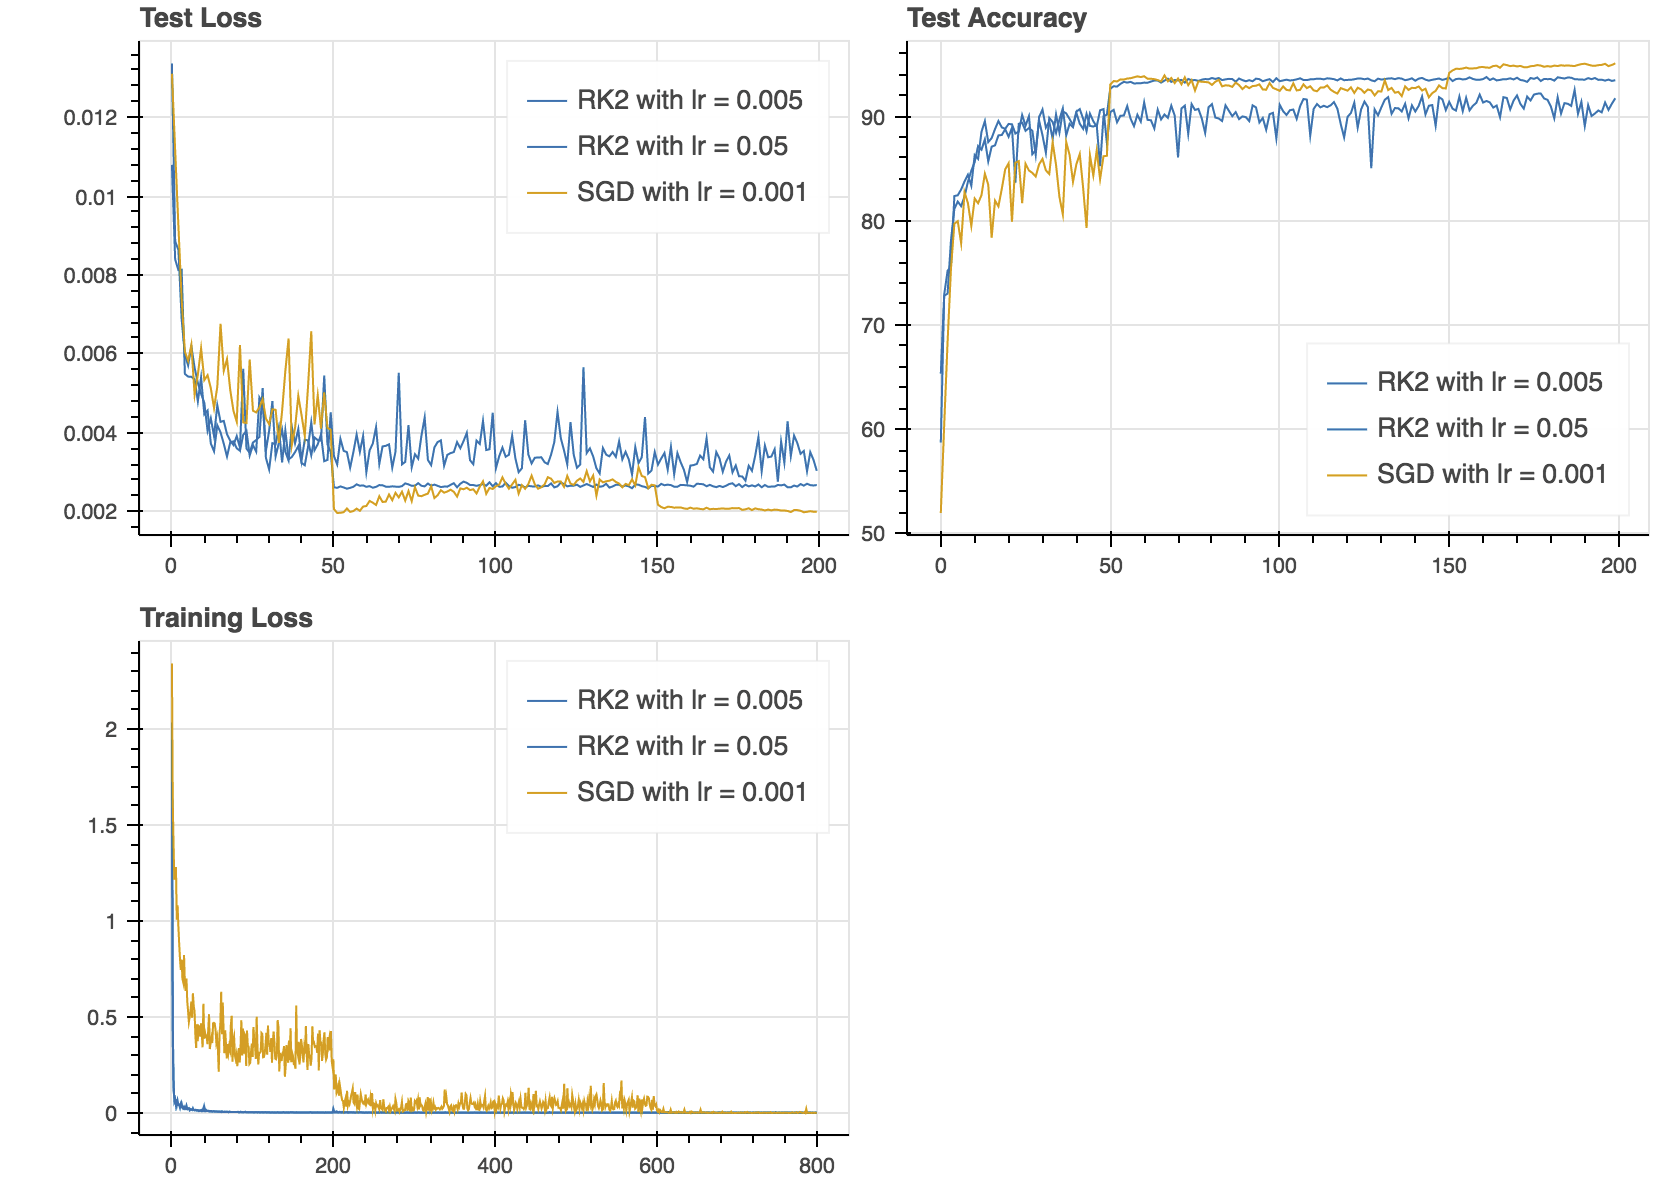
\includegraphics[scale=0.5]{cifar.png}
\textbf{WideResnet} -
Here we compare our optimization scheme, Runge-Kutta Ralston Method with Stochastic Gradient Descent.
\\
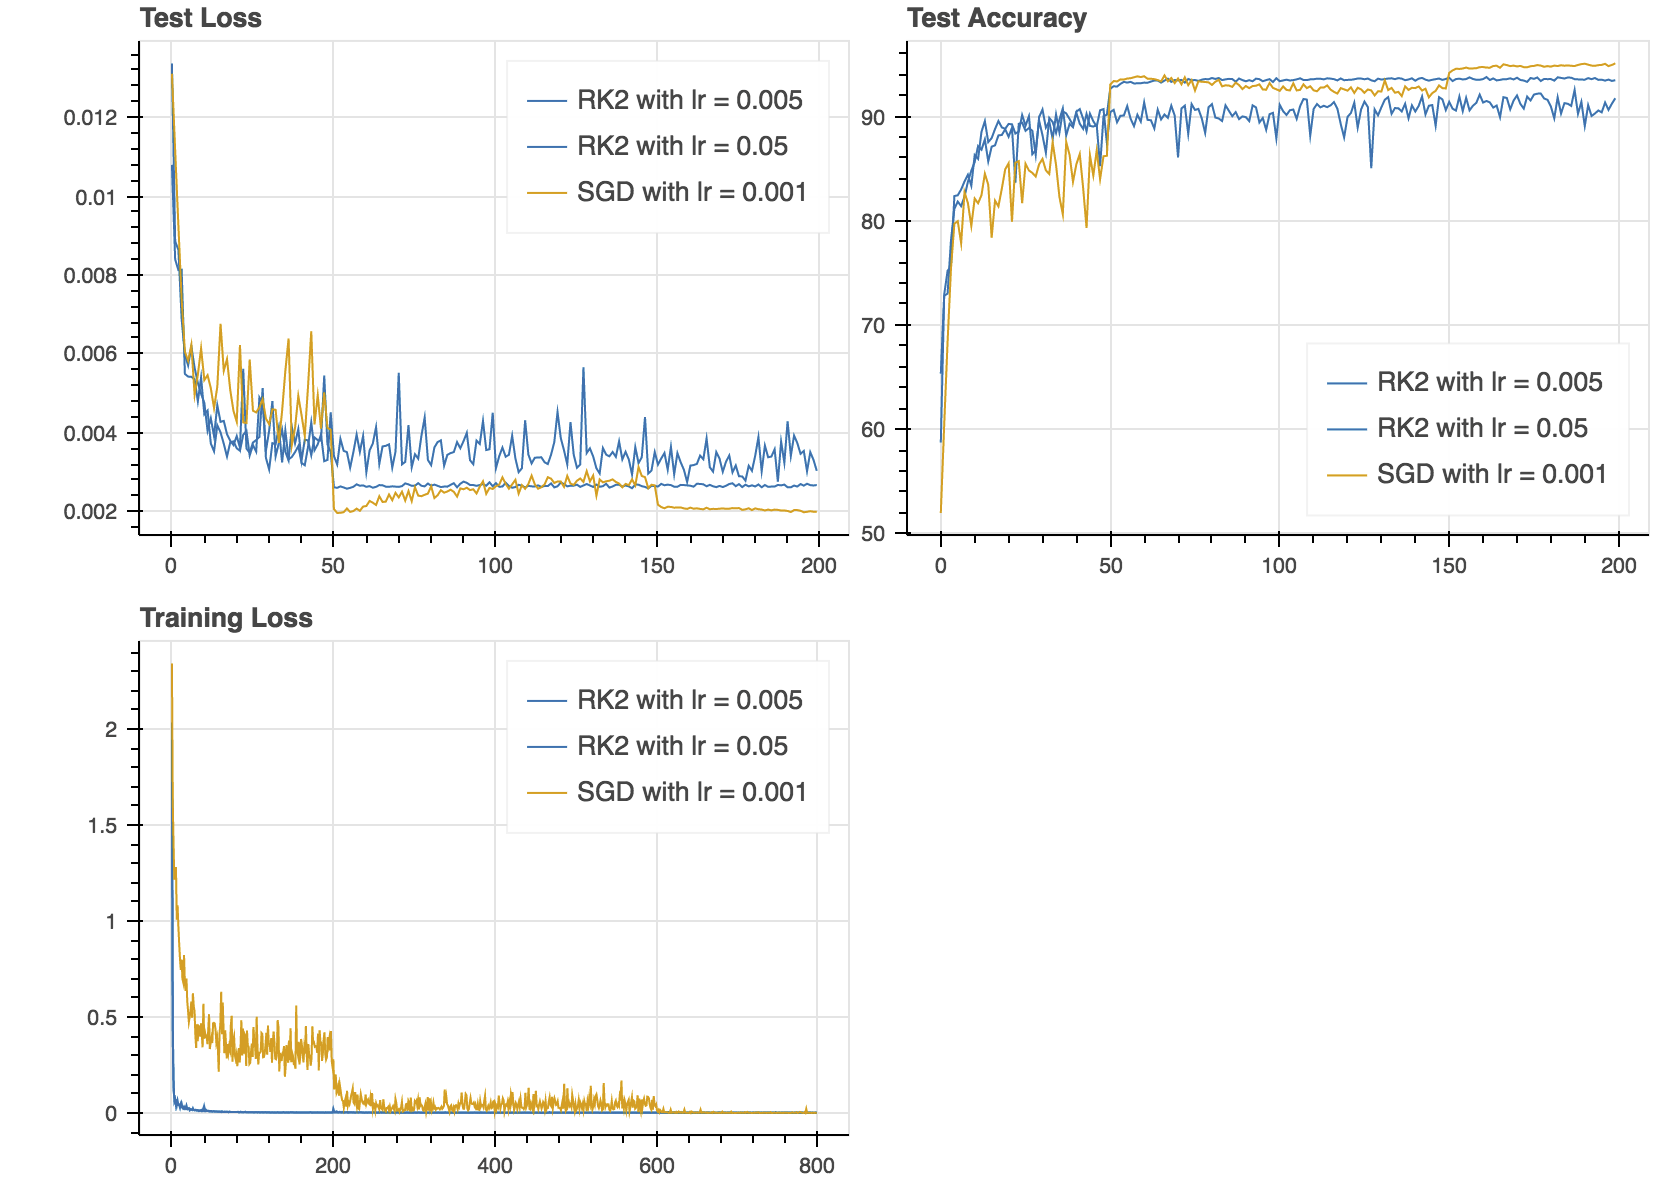
\includegraphics[scale=0.5]{wideresnet.png}

\subsection{Convex Models}


%!TEX root=./optim_report.tex
\subsection{Inequalities}
Here we present some common inequalities in convex analysis without proof, for proof refer to \cite{nesterov}
\begin{lemma}
Let $f : \mathbb{R}^d \rightarrow \mathbb{R}$  be convex and satisfy $|| \nabla f(x) - \nabla f(y) || \leq \beta || x -y ||$ for all $x,y \in \mathbb{R}^d$ . Then $\forall x,y \in \mathbb{R}^d$ the following are true:
\begin{align}
% 0 \leq f(x) - f(y) - \nabla f(y)^T (x-y) \leq \frac{\beta}{2} || x-y ||^2 \\
f(x) - f(y) \leq \nabla f(x)^T (x-y) - \frac{1}{2 \beta} || \nabla f(x) - \nabla f(y) ||^2 \\
\frac{1}{\beta} || \nabla f(x) - \nabla f(y) ||^2  \leq( \nabla f(x) - \nabla f(y))^T(x-y)
\end{align}
\end{lemma}
Now, for the class of Strongly Convex functions $\mathcal{S}_{\beta,\mu}^{k,p}(\mathbb{R}^n)$ we use the following inequalities:

\begin{equation}
\begin{aligned}
\left\langle \nabla f(x) -\nabla f(y), x-y \right\rangle \geq 0 \\
 0 \leq f(y) - f(x) -\nabla f(x)^T (y-x) \leq \frac{\beta}{2}||x-y||_2^2 \\
f(x) + \nabla f(x)^T (y-x) + \frac{1}{2\beta}||\nabla f(x)-\nabla f(y)||_2^2 \leq f(y) \\
\frac{1}{\beta}|| \nabla f(x)-\nabla f(y) ||_2^2 \leq(\nabla f(x)-\nabla f(y))^T(x-y) \leq \beta || x -y ||_2^2  \\
f(y) \geq f(x) + \nabla f(x)^T (y-x) + \frac{1}{2\mu}||y-x||_2^2
\end{aligned}
\end{equation}
Note, that $f(x) \geq f(x^*) + \frac{1}{2\mu}||x-x^*||_2^2 $
% \subsection{RK2-Heun}


% \subsection{Comparison to GD}



\end{document}
